\documentclass[12pt,a4paper,twoside]{article}

% Common preamble I use
\usepackage[utf8]{inputenc}         % Input encoding
\usepackage[T1]{fontenc}            % Font encoding
\usepackage{textcomp}               % Provides various additional symbols and text-related features
\usepackage{microtype}              % Improves micro-typography of the document
\usepackage{pifont}                 % Provides additional symbols, including dingbats
\usepackage{changepage}             % Allows adjustment of page layout parameters
\usepackage{ftnxtra}

\usepackage{chemgreek,textgreek}    % Greek letters 

\usepackage{authblk}                % For customizing author block layout in the title page

\usepackage{listings}               % Code listings
\usepackage{xcolor}                 % Color support

\usepackage{graphicx}               % Graphics support
\usepackage[top=2.5cm,bottom=2.5cm,left=2.5cm,right=2.5cm]{geometry}
\usepackage{tikz}                   % For in-doc drawings
\usepackage{subcaption}             % Enhanced support for sub-figures and sub-captions
\usepackage{amsmath}                % Math support
\usepackage{mathenv}                % Provides additional math environments
\usepackage{amssymb}                % Provides various additional mathematical symbols
\usepackage{amsthm}                 % Provides enhanced support for theorem-like environments
\usepackage{wrapfig}

\usepackage{xtab}                   % Tables with adjustable width 
\usepackage{multirow}               % For multi-row cells in tables
\usepackage{array}                  % Provides more flexible and customizable array and tabular environments
\usepackage{longtable}              % Allows tables that span multiple pages

\usepackage{booktabs}               % Enhanced tables
\usepackage{csquotes}               % Quotation marks
\usepackage{algorithmic}            % For typesetting algorithms
\usepackage{caption}                % Customizes captions in floating environments
\usepackage{subcaption}
\usepackage{ragged2e}               % Enhanced text alignment commands

\usepackage{enumitem}               % Customizable lists     

\usepackage[sort&compress]{natbib}  % Cite style
\setcitestyle{numbers,square,comma}

\usepackage{times}                  % Times font       

\usepackage{hyperref}               % Hyperlinks
\usepackage{url}                    % For typesetting URLs with line breaks at hyphens
\def\UrlBreaks{\do\/\do-}
\hypersetup{breaklinks=true}
\urlstyle{same}
\DeclareUrlCommand\email{}          % Email command
\usepackage{nameref}                % Enables referencing section names instead of numbers
  
\usepackage{algorithmic}            % For typesetting algorithms

% For using TODO notes
% \todo[inline,caption={}]{TODOs are to be inserted like this}
\usepackage[color=blue!10,textsize=footnotesize,textwidth=25mm]{todonotes}
% \usepackage[disable]{todonotes}
\usepackage{float}


\makeatletter
% Commands to format a counter value as Greek letter to be used like 
% \arabic or \roman:
\newcommand*\alphgreek[1]{\expandafter\@alphgreek\csname c@#1\endcsname}
\newcommand*\@alphgreek[1]{\csname chemgreekIntToGreek:n\endcsname{#1}}
\newcommand*\Alphgreek[1]{\expandafter\@Alphgreek\csname c@#1\endcsname}
\newcommand*\@Alphgreek[1]{\csname chemgreekIntToGreek:n\endcsname{#1}}

% Register new counter formats to enumitem:
\AddEnumerateCounter*{\alphgreek}{\@alphgreek}{\chemalpha}
\AddEnumerateCounter*{\Alphgreek}{\@Alphgreek}{\chemAlpha}
\makeatother

% \code{} command to insert in-text code snippets
\definecolor{light-gray}{gray}{0.95}
\newcommand{\code}[1]{\colorbox{light-gray}{\texttt{#1}}}

% AUTHORS
\newcommand{\Samuel}{Samuel Jonsson}
\newcommand{\SamuelMail}{sajs19@student.bth.se}

\newcommand{\Sri}{Sri Aditya Gundimeda}
\newcommand{\SriMail}{srgu22@student.bth.se}

% SUPERVISOR
\newcommand{\super}{Niklas Lavesson (NLA)} % Title Firstname Lastname
\newcommand{\superAffiliation}{Software Engineering (DIPT)} % Department; Computer Science, Mechanical Engineering, etc.
\newcommand{\superEmail}{niklas.lavesson@bth.se}

% REPORT METADATA
\newcommand{\thesisMonth}{Month}
\newcommand{\thesisYear}{2024}
\newcommand{\thesisWeeks}{20}
\newcommand{\thesisTitle}{Data analysis for Massive MIMO optimizations}
\newcommand{\thesisSubtitle}{Subtitle?}

\author{Samuel Jonsson}

\date{\today}

\title{MS1415: Assignment Report}

\begin{document}

\maketitle

\begin{figure}[!b]
    \centering
    
\includegraphics[width = 0.35\textwidth]{img/BTH_logo_black.png}
\end{figure}

\newpage

\section{Part 1}
\subsection{Plotting the combined observed signal}
\label{ssec:observedsignal}
% TODO:
% Define the tested regions;
% Create the observed signal with the vectorized pixels of these three regions using windows of 20 × 20 pixels;
% Check the data behavior to verify if the considered regression models are suitable approaches to fit such data;

I defined the three areas as squares of 20x20 and 40x40 pixels. The three areas were:

\begin{itemize}
    \item \code{A = (20:40, 20:40) \&\& (10:50, 10:50)}
    \item \code{B = (20:40, 320:340) \&\& (10:50, 310:350)}
    \item \code{C = (160:180, 320:340) \&\& (150:190, 310:350)}
\end{itemize}    
where \code{A} represents a sea-, \code{B} represents ground- and \code{C} represents city area.

\begin{figure}[!ht]
    \begin{subfigure}{.45\textwidth}
        \centering
        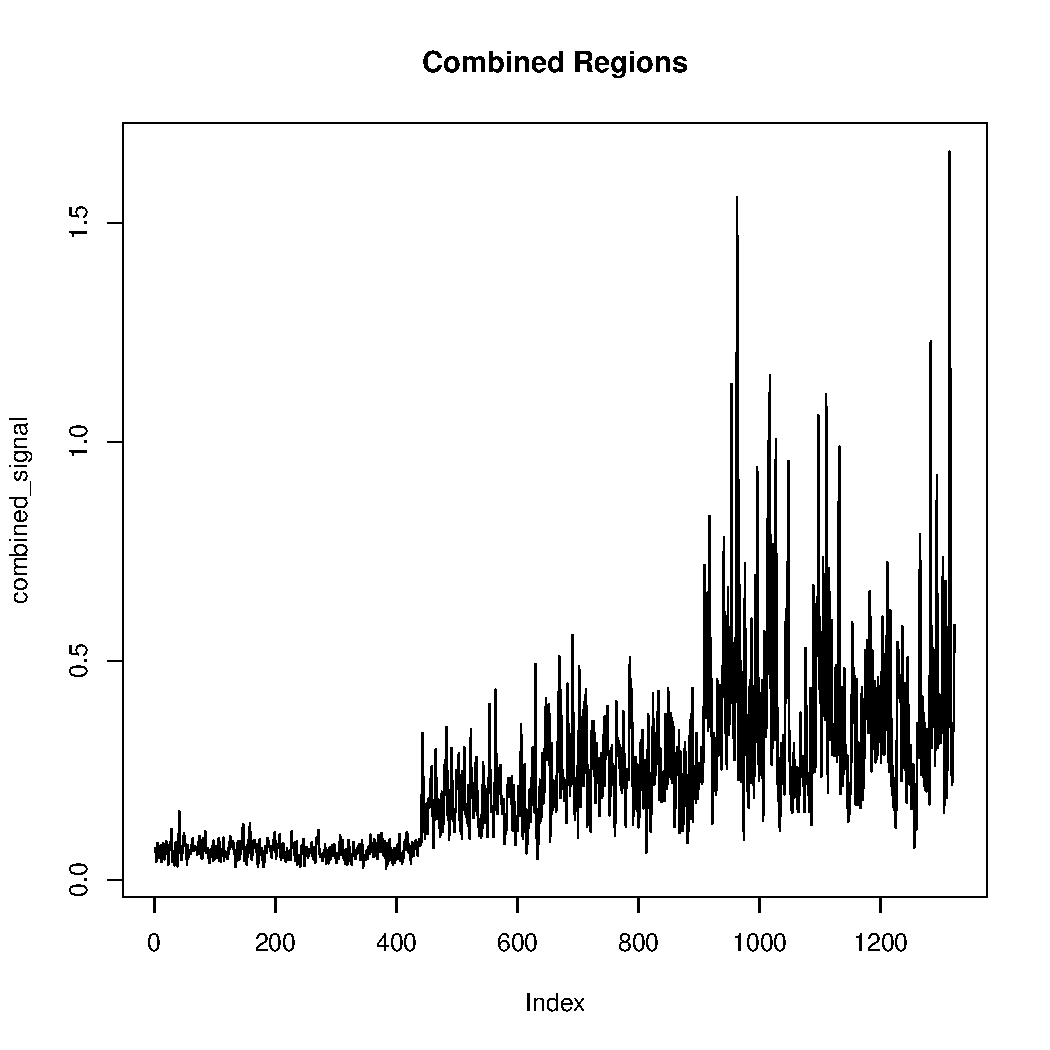
\includegraphics[width=\linewidth]{img/combined_regions_20x20.pdf}
        \caption{20x20}
        \label{fig:observededsignalfig20}
    \end{subfigure}
    \begin{subfigure}{.45\textwidth}
        \centering
        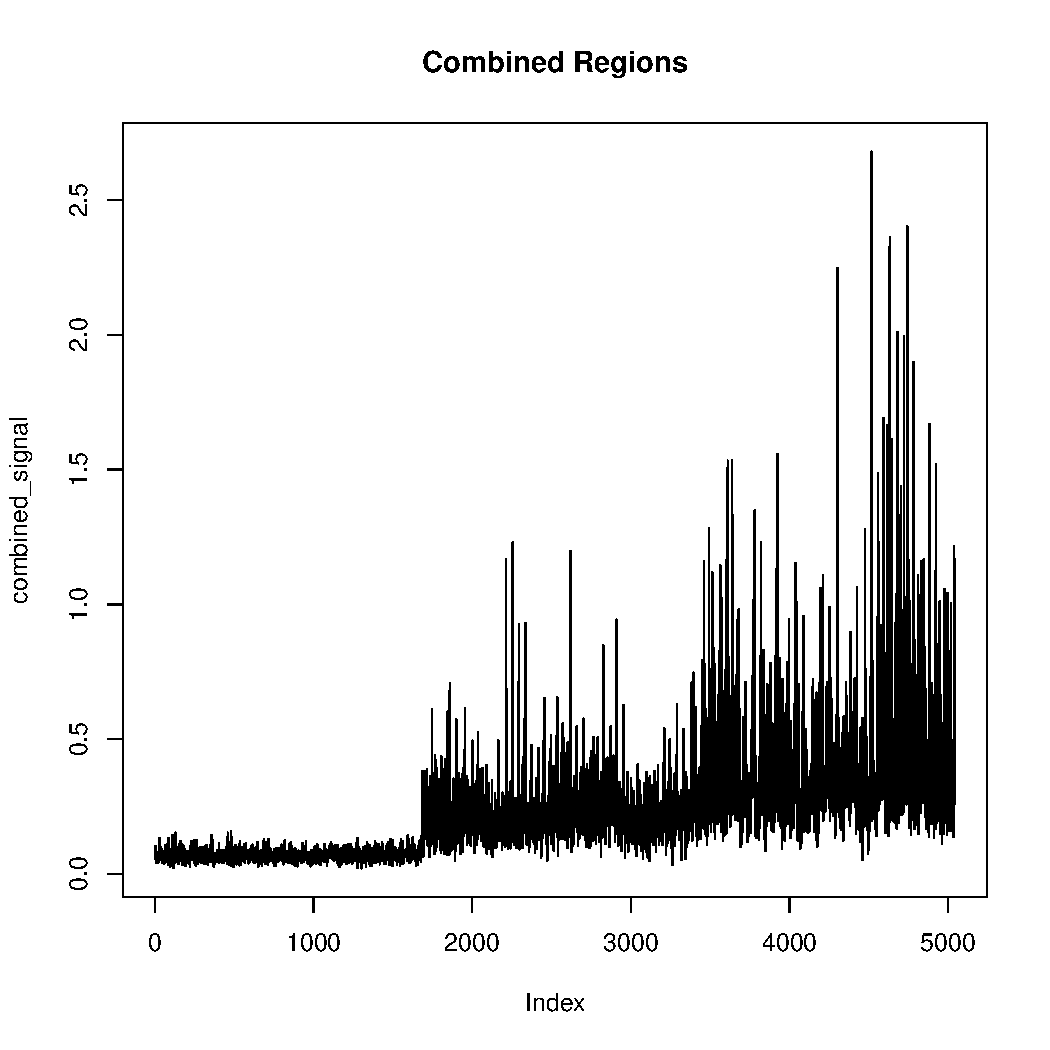
\includegraphics[width=\linewidth]{img/combined_regions_40x40.pdf}
        \caption{40x40}
        \label{fig:observededsignalfig40}
    \end{subfigure}
    \caption{The combined signals for the two region definitions}
    \label{fig:observededsignalfig}
\end{figure}

\noindent As one can observe in both Figure \ref{fig:observededsignalfig20} and Figure \ref{fig:observededsignalfig40},
the three areas \code{A}, \code{B} and \code{C} are all quite distinct in both plots, where \code{A} have little
activity and low average, while \code{B} and \code{C} have more activity and higher average. meanwhile, \code{C}
have more activity than \code{B}, which is understandable, considering a city square would contain more activity than a
ground square.

\newpage

\subsection{Modeling}
\label{ssec:modeling}
% TODO:
% Fit the selected regression models. You can use the functions available on Canvas.
% Perform the detection theory. Are the covariates significant to the model? Are they introducing information about variations in y?
% Test the residuals. Is the model correctly specified? (Consider a residual vs index plot and check evidence of normality with a histogram, for example).
% Verify the determination coefficient for the fitted models;

\subsubsection{Gamma distribution}
\label{sssec:gamma}
\begin{figure}[!ht]
    \begin{subfigure}{.45\textwidth}
        \centering
        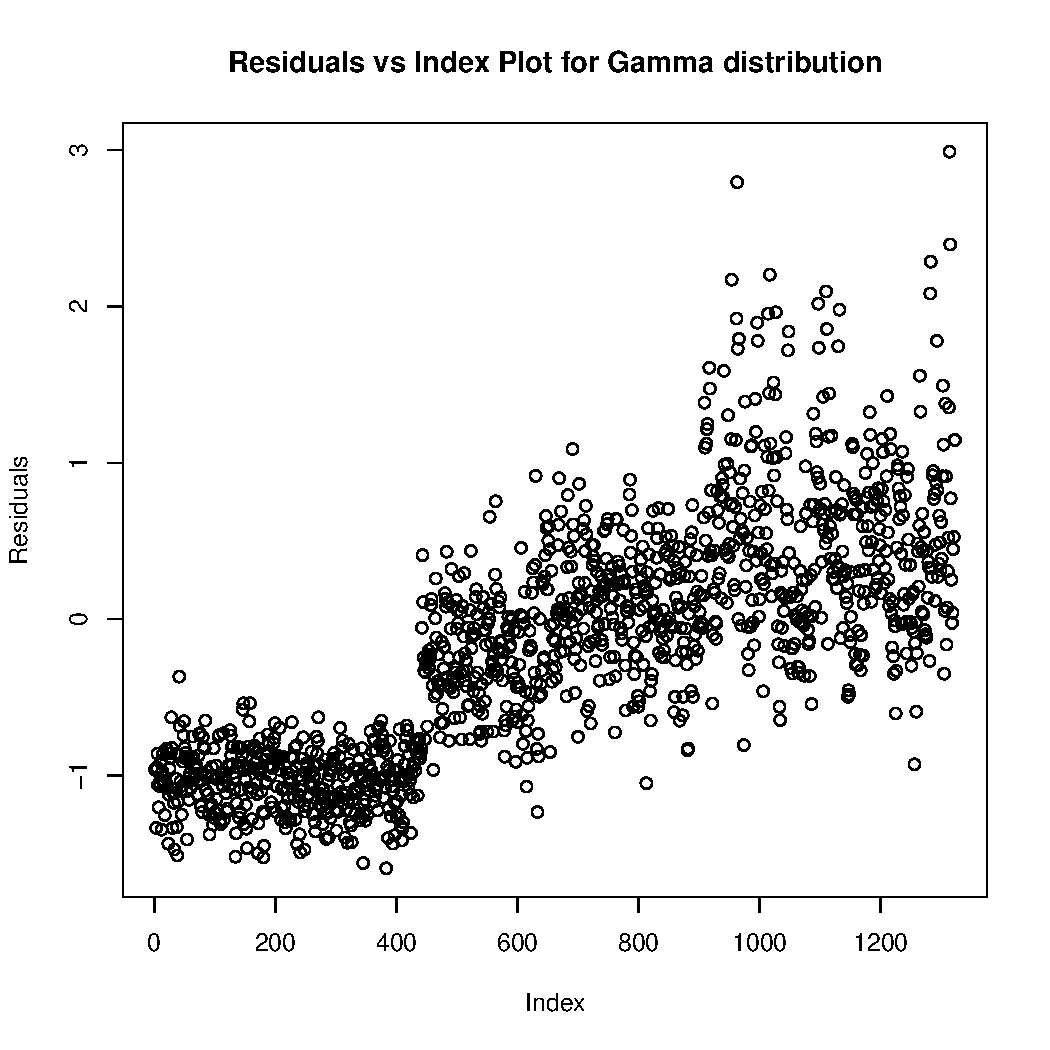
\includegraphics[width=\linewidth]{img/Gamma_distribution_20x20.pdf}
        \caption{Scatter plot of the residuals}
        \label{fig:gammascatter20}
    \end{subfigure}
    \begin{subfigure}{.45\textwidth}
        \centering
        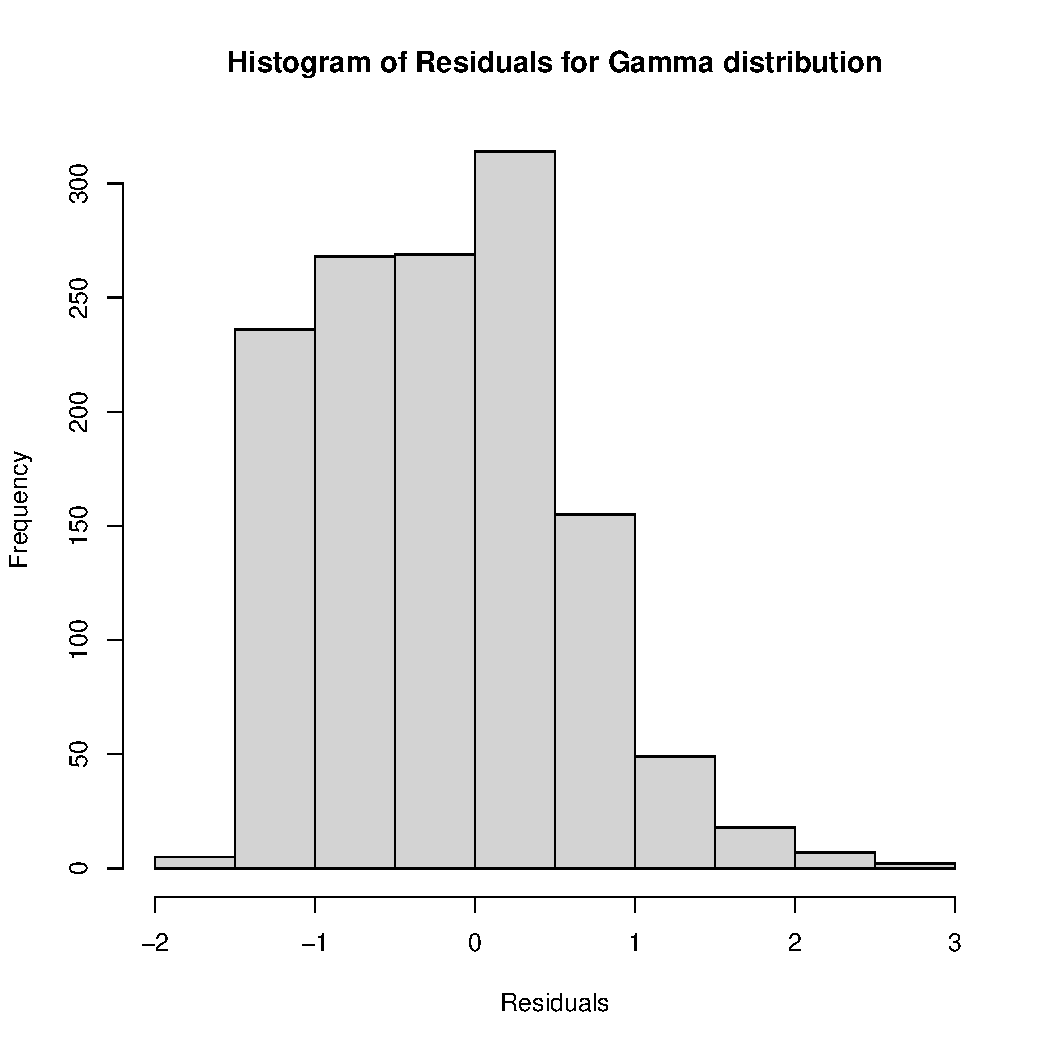
\includegraphics[width=\linewidth]{img/Gamma_distribution_histogram_20x20.pdf}
        \caption{Histogram plot of the distribution of residuals}
        \label{fig:gammahist20}
    \end{subfigure}
    \caption{A graphic representation of the residuals of the GLM model with Gamma
    distribution for areas of size 20x20}
    \label{fig:gammafig20}
\end{figure}

\begin{figure}[!ht]
    \begin{subfigure}{.45\textwidth}
        \centering
        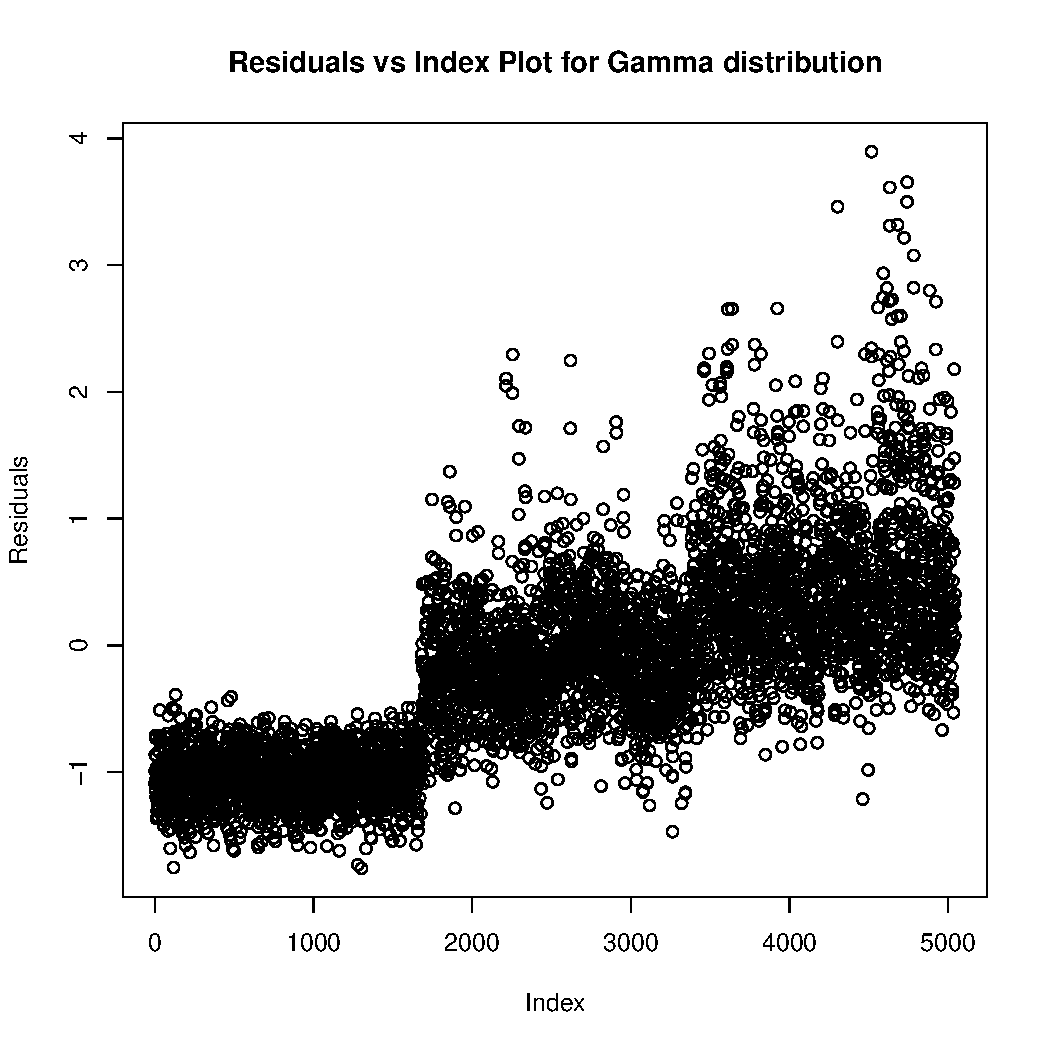
\includegraphics[width=\linewidth]{img/Gamma_distribution_40x40.pdf}
        \caption{Scatter plot of the residuals}
        \label{fig:gammascatter40}
    \end{subfigure}
    \begin{subfigure}{.45\textwidth}
        \centering
        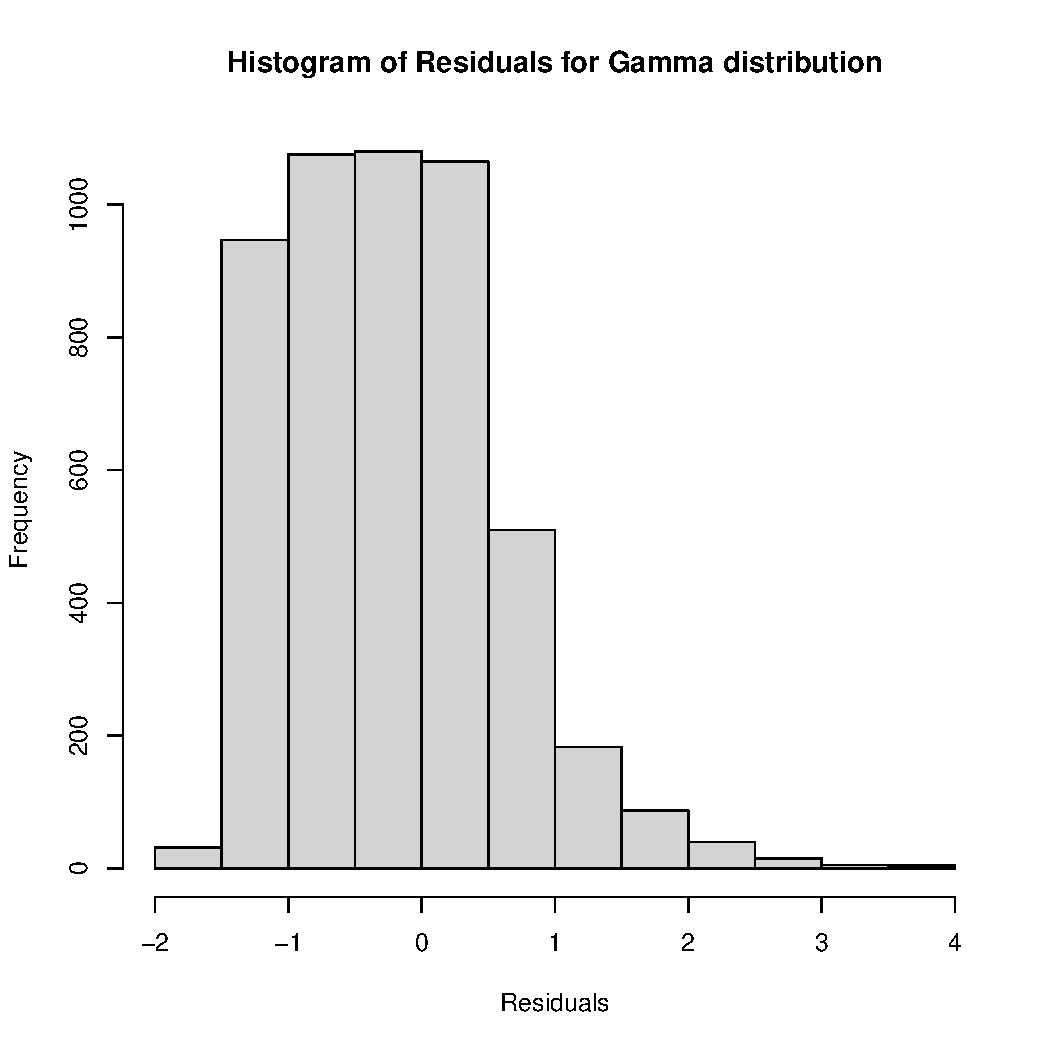
\includegraphics[width=\linewidth]{img/Gamma_distribution_histogram_40x40.pdf}
        \caption{Histogram plot of the distribution of residuals}
        \label{fig:gammahist40}
    \end{subfigure}
    \caption{A graphic representation of the residuals of the GLM model with Gamma
    distribution for areas of size 40x40}
    \label{fig:gammafig40}
\end{figure}

\newpage

\begin{longtable}{l|p{0.2\textwidth}|p{0.2\textwidth}|p{0.1\textwidth}|p{0.1\textwidth}|p{0.1\textwidth}}
	\textbf{Model} & \multicolumn{5}{r}{GLM with Gamma distribution}                                                             \\
	\hline
	\endhead
	\hline
	\multicolumn{6}{r}{\emph{Continued on the next page}}                                                                        \\
	\endfoot
	\hline
	\endlastfoot
	\hline
	\textbf{Dimensions} & \textbf{Parameter} & \textbf{Estimate Std.}   & \textbf{Error}  & \textbf{t-value} & \textbf{Pr(>|t|)} \\
    \hline
	(20x20)             & intercept          & -1.47672                 &  0.03974        & -37.161          &  <2e-16           \\
                        & x2                 &  0.02071                 &  0.05620        &  0.368           &  0.713            \\
                        & x3                 & -0.02717                 &  0.05620        & -0.484           &  0.629            \\
    \hline
    (40x40)             & intercept          & -1.46175                 &  0.02324        & -62.897          &  <2e-16           \\
                        & x2                 &  0.03720                 &  0.03287        &  1.132           &  0.258            \\
                        & x3                 &  0.05076                 &  0.03287        &  1.544           &  0.123            \\
    \caption{GLM model with Gamma distribution summary}
	\label{tab:gammasumtab}
\end{longtable}

\begin{longtable}{l|p{0.1\textwidth}|p{0.11\textwidth}|p{0.11\textwidth}|p{0.23\textwidth}|p{0.15\textwidth}}
	\textbf{Model} & \multicolumn{4}{r}{GLM with Gamma distribution } \\
	\hline
	\endhead
	\hline
	\multicolumn{5}{r}{\emph{Continued on the next page}} \\
	\endfoot
	\hline
	\endlastfoot
	\hline
	\textbf{Dimensions} & \textbf{std.}        & \textbf{Mean}        & \textbf{Median}        & \textbf{Min, Max}            & \textbf{$R^2$} \\
    \hline
    (20x20)             & \small 0.7642889     & \small -0.2006474    & \small -0.1716648      & \small (-1.592788, 2.989338) & 0.0006688601   \\
    \hline
    (40x40)             & \small 0.7974549     & \small -0.2227975    & \small -0.2480939      & \small (-1.759994, 3.896083) & 0.0006150857   \\
	\caption{GLM model with Gamma distribution distribution variables}
	\label{tab:gammavaltab}
\end{longtable}

\newpage

\subsubsection{Reyleigh distribution plots, devianvce residuals}
\label{sssec:reyleighdeviance}
\begin{figure}[!ht]
    \begin{subfigure}{.45\textwidth}
        \centering
        \includegraphics[width=\linewidth]{img/Reyleigh_distribution,_deviance_residuals_20x20.pdf}
        \caption{Scatter plot of the residuals}
        \label{fig:reyleighdeviancescatter20}
    \end{subfigure}
    \begin{subfigure}{.45\textwidth}
        \centering
        \includegraphics[width=\linewidth]{img/Reyleigh_distribution,_deviance_residuals_histogram_20x20.pdf}
        \caption{Histogram plot of the distribution of residuals}
        \label{fig:reyleighdeviancehist20}
    \end{subfigure}
    \caption{A graphic representation of the deviance residuals of the model with Reyleigh
    distributions for areas of size 40x40}
    \label{fig:reyleighdeviancefig20}
\end{figure}

\begin{figure}[!ht]
    \begin{subfigure}{.45\textwidth}
        \centering
        \includegraphics[width=\linewidth]{img/Reyleigh_distribution,_deviance_residuals_40x40.pdf}
        \caption{Scatter plot of the residuals}
        \label{fig:reyleighdeviancescatter40}
    \end{subfigure}
    \begin{subfigure}{.45\textwidth}
        \centering
        \includegraphics[width=\linewidth]{img/Reyleigh_distribution,_deviance_residuals_histogram_40x40.pdf}
        \caption{Histogram plot of the distribution of residuals}
        \label{fig:reyleighdeviancehist40}
    \end{subfigure}
    \caption{A graphic representation of the deviance residuals of the model with Reyleigh
    distributions for areas of size 40x40}
    \label{fig:reyleighdeviancefig40}
\end{figure}

\newpage

\subsubsection{Reyleigh distribution plots, with quantile residuals}
\label{sssec:reyleighquantile}
\begin{figure}[!ht]
    \begin{subfigure}{.45\textwidth}
        \centering
        \includegraphics[width=\linewidth]{img/Reyleigh_distribution,_quantile_residuals_20x20.pdf}
        \caption{Scatter plot of the residuals}
        \label{fig:reyleighquantilescatter20}
    \end{subfigure}
    \begin{subfigure}{.45\textwidth}
        \centering
        \includegraphics[width=\linewidth]{img/Reyleigh_distribution,_quantile_residuals_histogram_20x20.pdf}
        \caption{Histogram plot of the distribution of residuals}
        \label{fig:reyleighquantilehist20}
    \end{subfigure}
    \caption{A graphic representation of the quantile residuals of the model with Reyleigh
    distribution for areas of size 20x20}
    \label{fig:reyleighquantilefig20}
\end{figure}

\begin{figure}[!ht]
    \begin{subfigure}{.45\textwidth}
        \centering
        \includegraphics[width=\linewidth]{img/Reyleigh_distribution,_quantile_residuals_40x40.pdf}
        \caption{Scatter plot of the residuals}
        \label{fig:reyleighquantilescatter40}
    \end{subfigure}
    \begin{subfigure}{.45\textwidth}
        \centering
        \includegraphics[width=\linewidth]{img/Reyleigh_distribution,_quantile_residuals_histogram_40x40.pdf}
        \caption{Histogram plot of the distribution of residuals}
        \label{fig:reyleighquantilehist40}
    \end{subfigure}
    \caption{A graphic representation of the quantile residuals of the model with Reyleigh
    distribution for areas of size 40x40}
    \label{fig:reyleighquantilefig40}
\end{figure}

\newpage

\subsubsection{Reyleigh distribution plots, with standardized residuals}
\label{sssec:reyleighstandardized}
\begin{figure}[!ht]
    \begin{subfigure}{.45\textwidth}
        \centering
        \includegraphics[width=\linewidth]{img/Reyleigh_distribution,_quantile_residuals_20x20.pdf}
        \caption{Scatter plot of the residuals}
        \label{fig:reyleighstandardizedscatter20}
    \end{subfigure}
    \begin{subfigure}{.45\textwidth}
        \centering
        \includegraphics[width=\linewidth]{img/Reyleigh_distribution,_standardized_residuals_histogram_20x20.pdf}
        \caption{Histogram plot of the distribution of residuals}
        \label{fig:reyleighstandardizedhist20}
    \end{subfigure}
    \caption{A graphic representation of the standardized residuals of the model with Reyleigh
    distribution for areas of size 20x20}
    \label{fig:reyleighstandardizedfig20}
\end{figure}

\begin{figure}[!ht]
    \begin{subfigure}{.45\textwidth}
        \centering
        \includegraphics[width=\linewidth]{img/Reyleigh_distribution,_standardized_residuals_40x40.pdf}
        \caption{Scatter plot of the residuals}
        \label{fig:reyleighstandardizedscatter40}
    \end{subfigure}
    \begin{subfigure}{.45\textwidth}
        \centering
        \includegraphics[width=\linewidth]{img/Reyleigh_distribution,_standardized_residuals_histogram_40x40.pdf}
        \caption{Histogram plot of the distribution of residuals}
        \label{fig:reyleighstandardizedhist40}
    \end{subfigure}
    \caption{A graphic representation of the quantile residuals of the model with Reyleigh
    distribution for areas of size 40x40}
    \label{fig:reyleighstandardizedfig40}
\end{figure}

\newpage

\subsubsection{Reyleigh distribution tables}
\begin{longtable}{l|p{0.2\textwidth}|p{0.2\textwidth}|p{0.1\textwidth}|p{0.1\textwidth}|p{0.1\textwidth}}
	\textbf{Model} & \multicolumn{5}{r}{Reyleigh distribution} \\
	\hline
	\endhead
	\hline
	\multicolumn{6}{r}{\emph{Continued on the next page}}                                                                                         \\
	\endfoot
	\hline
	\endlastfoot
	\hline
	\textbf{Dimensions} & \textbf{Parameter} & \textbf{Estimate Std.}   & \textbf{Error}  & \textbf{t-value} & \textbf{Pr(>|t|)} \\
    \hline
	(20x20)             & intercept          & -1.3286                  &  0.0238         &  55.8016         &  0.0000           \\
                        & x2                 &  0.0171                  &  0.0337         &  0.5084          &  0.6111           \\
                        & x3                 & -0.0389                  &  0.0337         &  1.1566          &  0.2474           \\
    \hline
    (40x40)             & intercept          & -1.2688                  &  0.0122         &  104.0398        &  0.0000           \\
                        & x2                 &  0.0598                  &  0.0172         &  3.4694          &  0.0005           \\
                        & x3                 &  0.0552                  &  0.0172         &  3.2003          &  0.0014           \\
    \caption{Reyleigh distribution summary}
	\label{tab:reyleighsumtab}
\end{longtable}

\begin{longtable}{l|p{0.25\textwidth}|p{0.25\textwidth}|p{0.25\textwidth}}
	\textbf{Model} & \multicolumn{3}{r}{Reyleigh distribution, deviance residuals} \\
	\hline
	\endhead
	\hline
	\multicolumn{4}{r}{\emph{Continued on the next page}} \\
	\endfoot
	\hline
	\endlastfoot
	\hline
	\textbf{Dimensions} & \textbf{Residual type} & \textbf{Variable}      & \textbf{Value}         \\
    (20x20)             & Quantile               & \textbf{std.}          &  NaN                   \\
                        &                        & \textbf{Mean}          &  Inf                   \\
                        &                        & \textbf{Median}        & -0.6151298             \\
                        &                        & \textbf{Min, Max}      & (-2.679131, inf)       \\
                        &                        & \textbf{$R^2$}         &  NULL                  \\
    \hline
    (40x40)             & Quantile               & \textbf{std.}          &  NaN                   \\
                        &                        & \textbf{Mean}          &  Inf                   \\
                        &                        & \textbf{Median}        & -0.6151298             \\
                        &                        & \textbf{Min, Max}      & (-2.679131, Inf)       \\
                        &                        & \textbf{$R^2$}         &  NULL                  \\
    \hline
    (20x20)             & Standardized           & \textbf{std.}          &  1.38259               \\
                        &                        & \textbf{Mean}          & -0.2548758             \\
                        &                        & \textbf{Median}        & -0.526009              \\
                        &                        & \textbf{Min, Max}      & (-1.72133, 10.57335)   \\
                        &                        & \textbf{$R^2$}         & NULL                   \\
    \hline
    (40x40)             & Standardized           & \textbf{std.}          &  1.488796              \\
                        &                        & \textbf{Mean}          & -0.3498187             \\
                        &                        & \textbf{Median}        & -0.7040906             \\
                        &                        & \textbf{Min, Max}      & (-1.781797, 15.33941)  \\
                        &                        & \textbf{$R^2$}         &  NULL                  \\
    \hline
    (20x20)             & Deviance               & \textbf{std.}          &  1.341344              \\
                        &                        & \textbf{Mean}          & -0.6748278             \\
                        &                        & \textbf{Median}        & -0.7355604             \\
                        &                        & \textbf{Min, Max}      & (-2.765231, 7.605446   \\
                        &                        & \textbf{$R^2$}         &  0.00218468701055219   \\
    \hline
    (40x40)             & Deviance               & \textbf{std.}          &  1.409814              \\
                        &                        & \textbf{Mean}          & -0.7901977             \\
                        &                        & \textbf{Median}        & -0.9446027             \\
                        &                        & \textbf{Min, Max}      &  (-3.025502, 10.83438) \\
                        &                        & \textbf{$R^2$}         &  0.00291242373199341   \\
    \caption{Reyleigh distribution distribution variables}
	\label{tab:gammavaltab}
\end{longtable}

\subsubsection{Normal distribution}
\label{sssec:gaussian}
\begin{figure}[!ht]
    \begin{subfigure}{.45\textwidth}
        \centering
        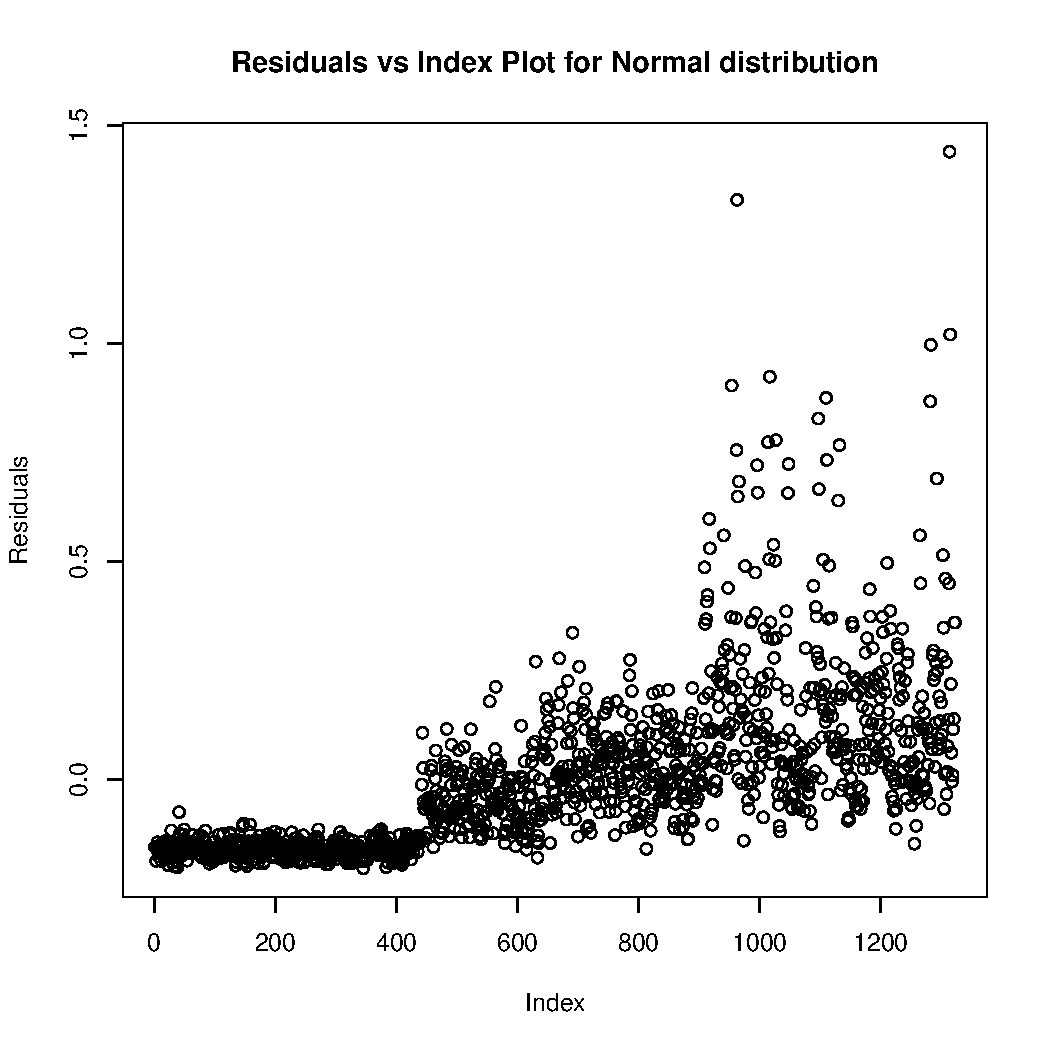
\includegraphics[width=\linewidth]{img/Normal_distribution_20x20.pdf}
        \caption{Scatter plot of the residuals}
        \label{fig:gaussianscatter20}
    \end{subfigure}
    \begin{subfigure}{.45\textwidth}
        \centering
        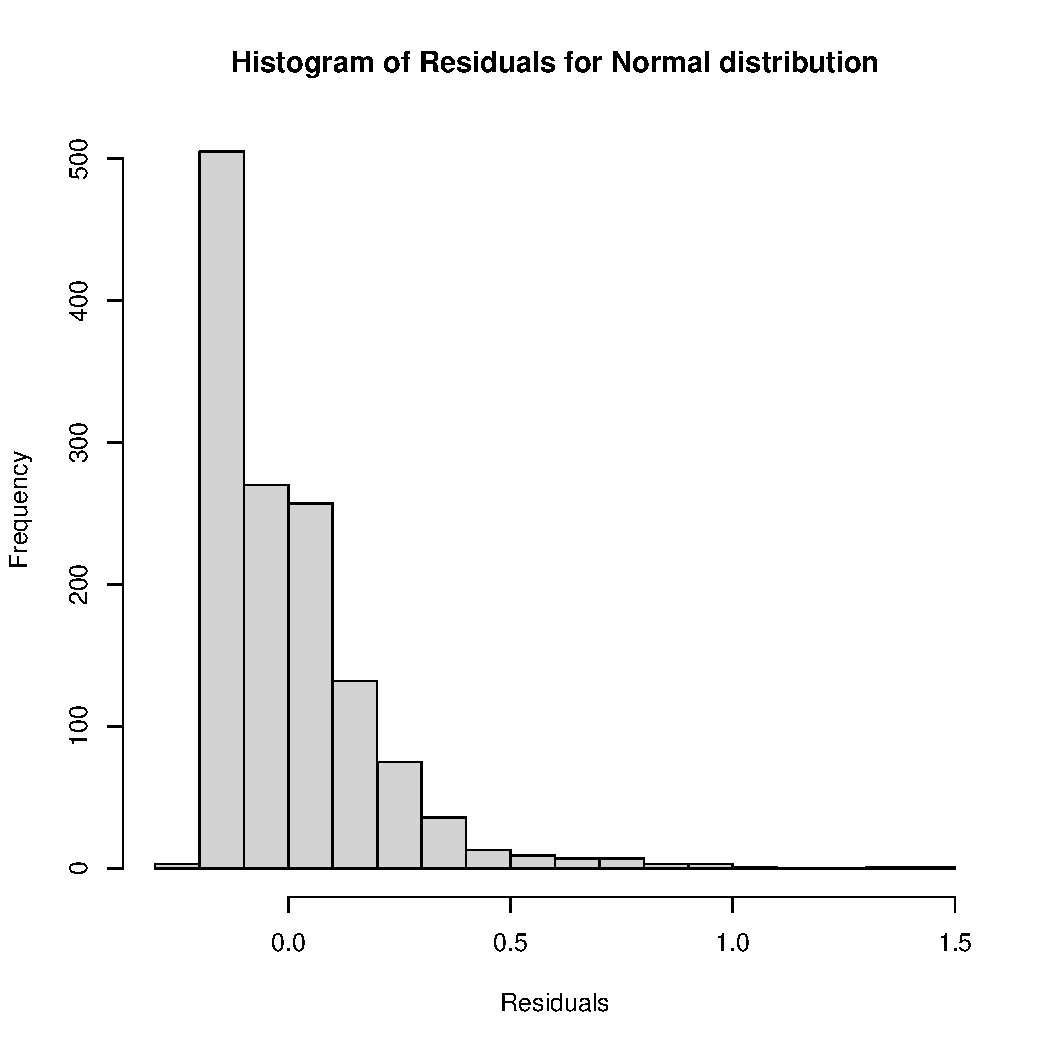
\includegraphics[width=\linewidth]{img/Normal_distribution_histogram_20x20.pdf}
        \caption{Histogram plot of the distribution of residuals}
        \label{fig:gaussianhist20}
    \end{subfigure}
    \caption{A graphic representation of the residuals of the GLM model with Normal (Gaussian)
    distribution for areas of size 20x20.}
    \label{fig:gaussianfig20}
\end{figure}

\begin{figure}[!ht]
    \begin{subfigure}{.45\textwidth}
        \centering
        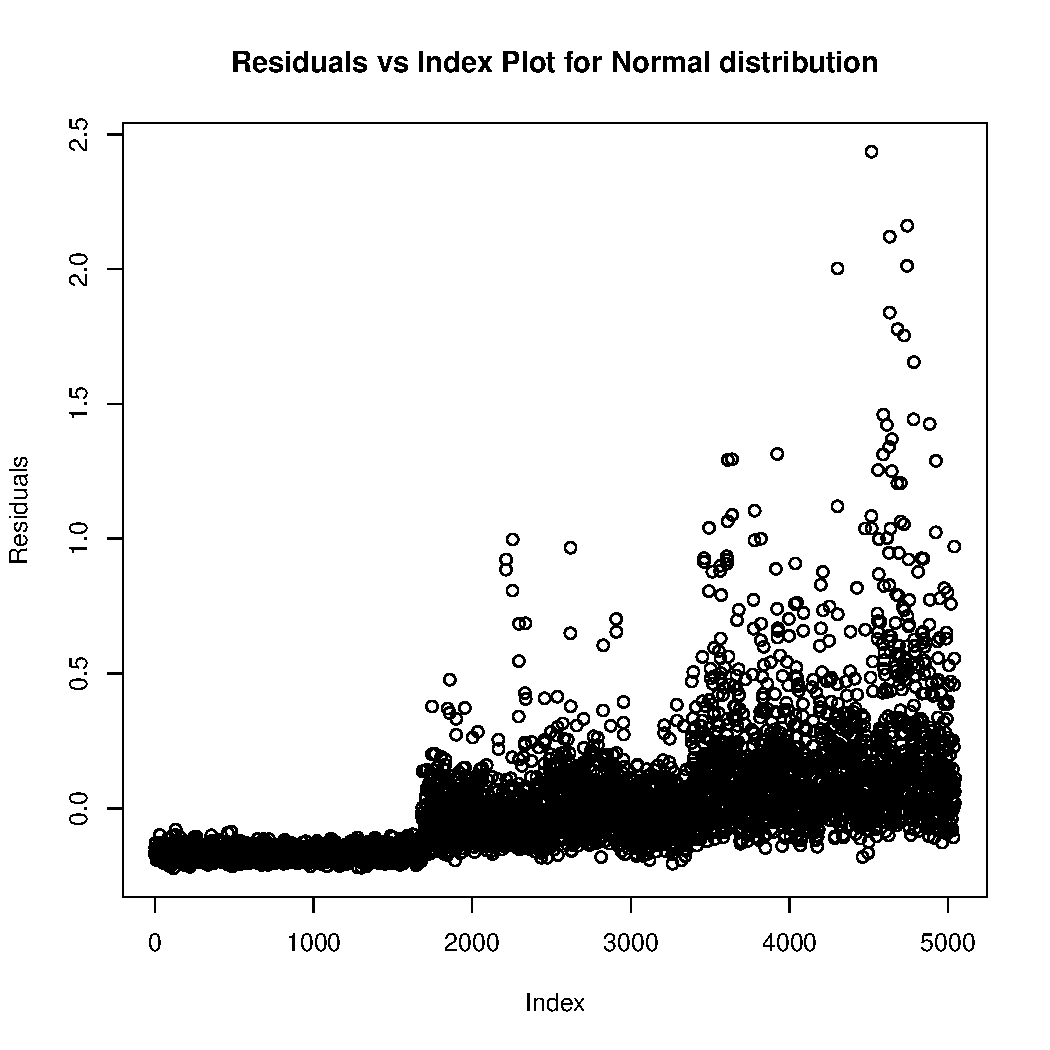
\includegraphics[width=\linewidth]{img/Normal_distribution_40x40.pdf}
        \caption{Scatter plot of the residuals}
        \label{fig:gaussianscatter40}
    \end{subfigure}
    \begin{subfigure}{.45\textwidth}
        \centering
        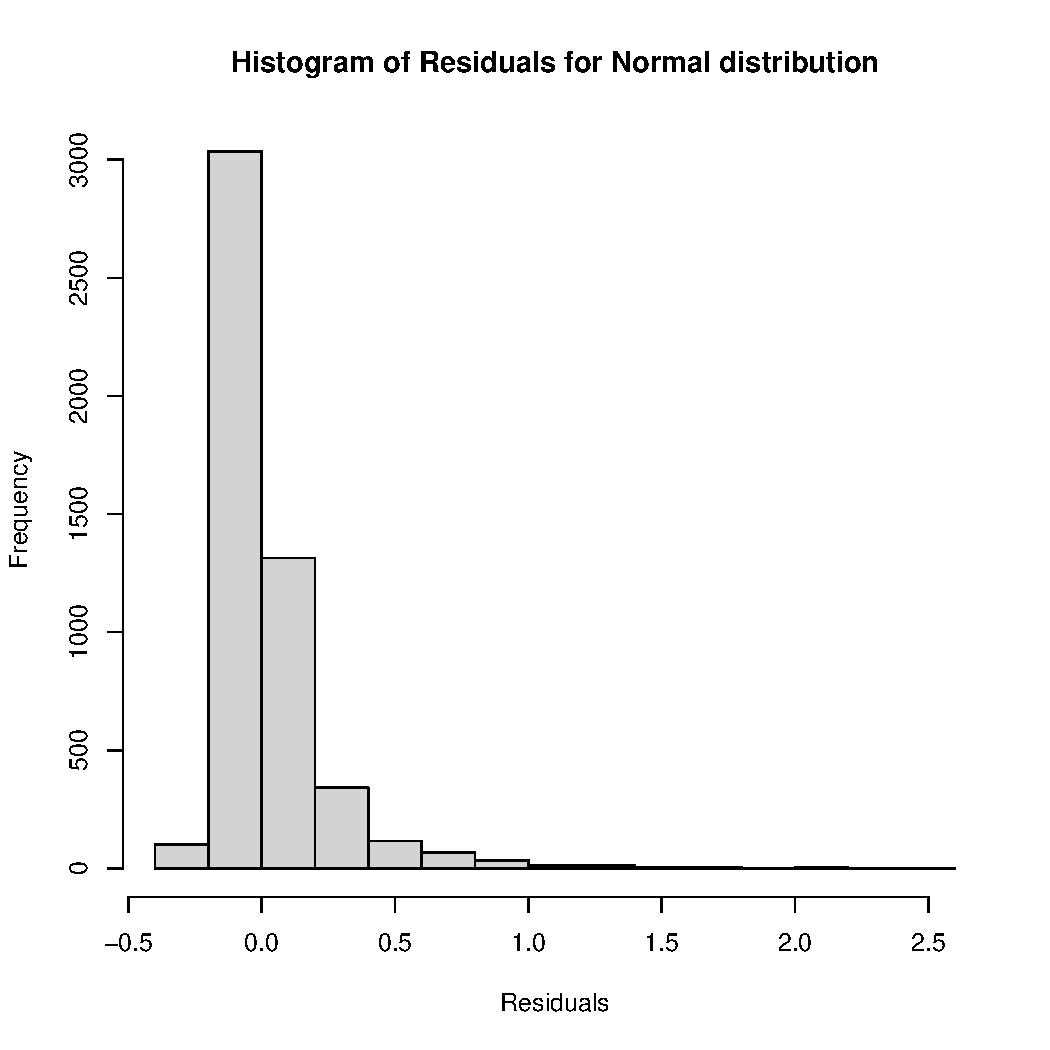
\includegraphics[width=\linewidth]{img/Normal_distribution_histogram_40x40.pdf}
        \caption{Histogram plot of the distribution of residuals}
        \label{fig:gaussianhist40}
    \end{subfigure}
    \caption{A graphic representation of the residuals of the GLM model with Normal (Gaussian)
    distribution for areas of size 40x40.}
    \label{fig:gaussianfig40}
\end{figure}

\begin{longtable}{l|p{0.2\textwidth}|p{0.2\textwidth}|p{0.1\textwidth}|p{0.1\textwidth}|p{0.1\textwidth}}
	\textbf{Model} & \multicolumn{2}{r}{GLM with Normal distribution} \\
	\hline
	\endhead
	\hline
	\multicolumn{3}{r}{\emph{Continued on the next page}}    \\
	\endfoot
	\hline
	\endlastfoot
	\hline
	\textbf{Dimensions} & \textbf{Parameter} & \textbf{Estimate Std.}   & \textbf{Error}  & \textbf{t-value} & \textbf{Pr(>|t|)} \\
    \hline
	(20x20)             & intercept          &  0.228385                &  0.009063       &  25.201          &  <2e-16           \\
                        & x2                 &  0.004779                &  0.012817       &  0.373           &  0.709            \\
                        & x3                 & -0.006123                &  0.012817       & -0.478           &  0.633            \\
    \hline
    (40x40)             & intercept          &  0.231831                &  0.005553       &  41.751          &  <2e-16           \\
                        & x2                 &  0.008788                &  0.007853       &  1.119           &  0.263            \\
                        & x3                 &  0.012071                &  0.007853       &  1.537           &  0.124            \\
	\caption{Normal distribution}
	\label{tab:gaussiantab}
\end{longtable}

\begin{longtable}{l|p{0.1\textwidth}|p{0.11\textwidth}|p{0.12\textwidth}|p{0.23\textwidth}|p{0.15\textwidth}}
	\textbf{Model} & \multicolumn{4}{r}{GLM with Normal distribution } \\
	\hline
	\endhead
	\hline
	\multicolumn{5}{r}{\emph{Continued on the next page}} \\
	\endfoot
	\hline
	\endlastfoot
	\hline
	\textbf{Dimensions} & \textbf{std.}    & \textbf{Mean}             & \textbf{Median}    & \textbf{Min, Max}             & \textbf{$R^2$} \\
    \hline
    (20x20)             & \small 0.1901713 & \scriptsize -5.953003e-17 & \small -0.03765383 & \small (-0.2043748, 1.440338) &  0.0005505713  \\
    \hline
    (40x40)             & \small 0.2276174 & \scriptsize -3.96736e-16  & \small -0.05413859 & \small (-0.2228668, 2.435698) & 0.0005010483   \\
	\caption{GLM model with Normal distribution distribution variables}
	\label{tab:gammavaltab}
\end{longtable}

\subsection{Conclusion}
\label{ssec:conclusion}
Looking at the results, there is only one setup that produces a somewhat good result, and that is the Reyleigh distribution and its deviance residuals.
Given that it is the only distribution where the residuals have a P value below 0.1, the other models are unlikely to produce any good results, and that
is only for the 40x40 pixel version of the model. It also is the one that has the best distribution of residuals.

Something to note, however, is that all models have an estimate below 0.1 for $x2$ and $x3$ and the $R^{2}$ for the Reyleigh distribution with deviance
residuals is only $\approx002912$ for the 40x40 sized squares, meaning the models does not account for a significant amount of the observed variability
in the data. Therefore, while it may have some utility, its explanatory power is quite limited. 

% What is the most accurate model for such data, considering detection and modeling evaluation?

\newpage
\section{Part 2}
\subsection{Results}
\begin{longtable}{l|p{0.3\textwidth}|p{0.2\textwidth}}
	\textbf{Layer} & \textbf{Output shape} & \textbf{Params} \\
	\hline
	\endhead
	\hline
	\multicolumn{3}{r}{\emph{Continued on the next page}}    \\
	\endfoot
	\hline
	\endlastfoot
	\hline
	 &  &  \\
	\caption{Part 2 result table}
	\label{tab:part2res}
\end{longtable}
\subsection{Analysis}

\end{document}